\documentclass[12pt,reqno]{amsart}

\usepackage{amsthm,amsmath,amssymb}
\usepackage{mathtools}
\usepackage{proof}
\usepackage{xcolor}
\usepackage{graphicx}
\usepackage[T1]{fontenc}
\usepackage{courier}
\usepackage{hyperref}
\hypersetup{
    hidelinks=true
}
\usepackage{array}
\usepackage{multirow}
\usepackage{listings}
\lstset{basicstyle=\ttfamily\tiny, columns=fullflexible, language=Python, morekeywords={logical_and, log, exp, dot, sqrt, ones, identity}}
\newcommand{\code}[1]{\texttt{#1}}
\newcommand\MyBox[2]{
  \fbox{\lower0.75cm
    \vbox to 1.7cm{\vfil
      \hbox to 1.7cm{\hfil\parbox{1.4cm}{#1\\#2}\hfil}
      \vfil}%
  }%
}
\graphicspath{ {./} }

\begin{document}

\begin{center}
\large\textbf{Assignment 2 \\ DASC521 Fall 2019} \\
\normalsize\textbf{Introduction to Machine Learning \\  Erhan Tezcan 0070881 \\ 18.10.2019} \\
\end{center}

\section{Task}
We are given 1000 images ($28\times28$ pixels $= 784$ pixels), each image belonging to one of 5 classes which are types of clothes. For the implementation, we mainly use methods specified in chapter 10.8 of the book ``Introduction to Machine Learning'' by Ethem Alpaydın. We will split the data in half, first 500 to be used for training and the remaining 500 to be used for testing.
\section{Implementation}
We are going to do Discriminaton by Regression for multiple classes. We will be using sigmoid function, which is defined as $\sigma: \mathbb{R} \xrightarrow{} (0, 1)$
\begin{equation}
\sigma(a) = \frac{1}{1 + e^{-a}}
\end{equation} 

In this case, we will apply sigmoid every element in the result $X.W + W_0$, where $X$ is the input matrix, where each row represents an image as an array of pixels, $W$ is the weight matrix and $W_0$ is the bias. \\

It is important to note that we do One-Hot Encoding to our labels before we proceed, so that we can compare them to our predictions. \\

The error function we use is the sum of squared errors:
\begin{equation}
\text{E}(w, w_0|X) = \frac{1}{2}\sum_t(r^t-y^t)^2
\end{equation}

We want to minimize this function, thus by using Gradient Descent we get the values below for adjusting weights and biases:
\begin{equation}
\Delta W = \eta \sum_t(r_i^t - y_i^t)\times y_i^t\times(1-y_i^t)\times x^t
\end{equation}
\begin{equation}
\Delta W_0 = \eta \sum_t(r_i^t - y_i^t)\times y_i^t\times(1-y_i^t)
\end{equation}

As stated in the book, after certain amount of iterations the correct label should have a larger predicted value, compared to rest, which we then find by taking the maximum of the predictions per class. Our loop has two termination conditions:
\begin{enumerate}
\item Maximum iteration count is reached.
\item The total change of $W$ and $W_0$ is less than some small $\epsilon$.
\end{enumerate}

We plot how the error changes by iteration, and we get the result below: \\
\begin{centering}
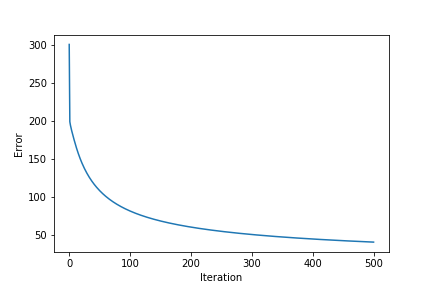
\includegraphics[width=0.6\textwidth]{plot.png}
\end{centering}

Overall, our accuracies are: 
\begin{itemize}
\item Training Data: $94\%$
\item Test Data: $93.2\%$
\end{itemize}
\end{document}